\documentclass[runningheads]{llncs}
\usepackage[T1]{fontenc}
\usepackage{graphicx}
\begin{document}
%
\title{Similarity Index of 1D Cellular Automata}

\author{Erick Jesse Angeles L\'opez\inst{1}}
%
\authorrunning{E. J. Angeles L\'opez}
% First names are abbreviated in the running head.
% If there are more than two authors, 'et al.' is used.
%
\institute{Instituto Polit\'ecnico Nacional, Escuela Superior de C\'omputo, Ciudad de M\'exico, M\'exico\\
\email{angeleslopezerickjesse@gmail.com}}
%
\maketitle              % typeset the header of the contribution
%
\begin{abstract}
The abstract should briefly summarize the contents of the paper in
150--250 words.

\keywords{Cellular Automata \and Similarity Index \and 1D Automata.}
\end{abstract}
%
%
%

\section{First Section2}
\subsection{A Subsection Sample}
Please note that the first paragraph of a section or subsection is
not indented. The first paragraph that follows a table, figure,
equation etc. does not need an indent, either.

Subsequent paragraphs, however, are indented.

\subsubsection{Sample Heading (Third Level)} Only two levels of
headings should be numbered. Lower level headings remain unnumbered;
they are formatted as run-in headings.

\paragraph{Sample Heading (Fourth Level)}
The contribution should contain no more than four levels of
headings. Table~\ref{tab1} gives a summary of all heading levels.

\begin{table}
	\caption{Table captions should be placed above the
		tables.}\label{tab1}
	\begin{tabular}{|l|l|l|}
		\hline
		Heading level &  Example & Font size and style\\
		\hline
		Title (centered) &  {\Large\bfseries Lecture Notes} & 14 point, bold\\
		1st-level heading &  {\large\bfseries 1 Introduction} & 12 point, bold\\
		2nd-level heading & {\bfseries 2.1 Printing Area} & 10 point, bold\\
		3rd-level heading & {\bfseries Run-in Heading in Bold.} Text follows & 10 point, bold\\
		4th-level heading & {\itshape Lowest Level Heading.} Text follows & 10 point, italic\\
		\hline
	\end{tabular}
\end{table}


\noindent Displayed equations are centered and set on a separate
line.
\begin{equation}
	x + y = z
\end{equation}
Please try to avoid rasterized images for line-art diagrams and
schemas. Whenever possible, use vector graphics instead (see
Fig.~\ref{fig1}).

\begin{figure}
	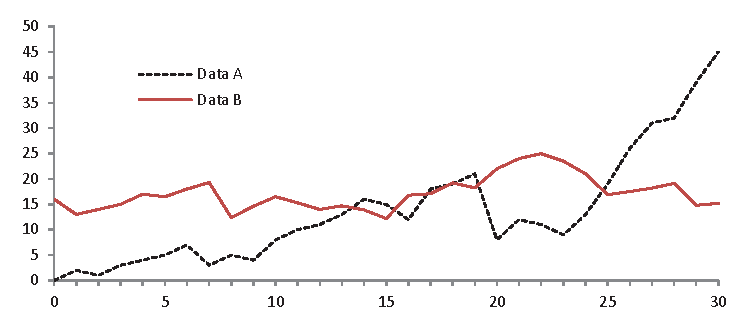
\includegraphics[width=\textwidth]{fig1.eps}
	\caption{A figure caption is always placed below the illustration.
		Please note that short captions are centered, while long ones are
		justified by the macro package automatically.} \label{fig1}
\end{figure}

\begin{theorem}
	This is a sample theorem. The run-in heading is set in bold, while
	the following text appears in italics. Definitions, lemmas,
	propositions, and corollaries are styled the same way.
\end{theorem}
%
% the environments 'definition', 'lemma', 'proposition', 'corollary',
% 'remark', and 'example' are defined in the LLNCS documentclass as well.
%
\begin{proof}
	Proofs, examples, and remarks have the initial word in italics,
	while the following text appears in normal font.
\end{proof}
For citations of references, we prefer the use of square brackets
and consecutive numbers. Citations using labels or the author/year
convention are also acceptable. The following bibliography provides
a sample reference list with entries for journal
articles~\cite{ref_article1}, an LNCS chapter~\cite{ref_lncs1}, a
book~\cite{ref_book1}, proceedings without editors~\cite{ref_proc1},
and a homepage~\cite{ref_url1}. Multiple citations are grouped
\cite{ref_article1,ref_lncs1,ref_book1},
\cite{ref_article1,ref_book1,ref_proc1,ref_url1}.

\begin{credits}
	\subsubsection{\ackname} The author thanks Sukanta Das for his mentorship and guidance
	throughout this research.
	
	\subsubsection{\discintname}
	It is now necessary to declare any competing interests or to specifically
	state that the authors have no competing interests. Please place the
	statement with a bold run-in heading in small font size beneath the
	(optional) acknowledgments\footnote{If EquinOCS, our proceedings submission
		system, is used, then the disclaimer can be provided directly in the system.},
	for example: The authors have no competing interests to declare that are
	relevant to the content of this article. Or: Author A has received research
	grants from Company W. Author B has received a speaker honorarium from
	Company X and owns stock in Company Y. Author C is a member of committee Z.
\end{credits}


%
% ---- Bibliography ----
%
% BibTeX users should specify bibliography style 'splncs04'.
% References will then be sorted and formatted in the correct style.
%
% \bibliographystyle{splncs04}
% \bibliography{mybibliography}
%
\begin{thebibliography}{8}
\bibitem{ref_article1}
Author, F.: Article title. Journal \textbf{2}(5), 99--110 (2016)

\bibitem{ref_lncs1}
Author, F., Author, S.: Title of a proceedings paper. In: Editor,
F., Editor, S. (eds.) CONFERENCE 2016, LNCS, vol. 9999, pp. 1--13.
Springer, Heidelberg (2016). \doi{10.10007/1234567890}

\bibitem{ref_book1}
Author, F., Author, S., Author, T.: Book title. 2nd edn. Publisher,
Location (1999)

\bibitem{ref_proc1}
Author, A.-B.: Contribution title. In: 9th International Proceedings
on Proceedings, pp. 1--2. Publisher, Location (2010)

\bibitem{ref_url1}
LNCS Homepage, \url{http://www.springer.com/lncs}, last accessed 2023/10/25
\end{thebibliography}
\end{document}
